\documentclass[a4paper]{report}

% Packages
\usepackage{graphicx}
\usepackage{epsfig}
\usepackage{pdflscape}
\usepackage{rotating}
\usepackage{listings}
\usepackage{multirow}
\usepackage{multicol}
\lstset{numbers=right, 
                numberstyle=\tiny, 
                breaklines=true,
                backgroundcolor=\color{light-gray},
                numbersep=5pt,
                xleftmargin=.25in,
                xrightmargin=.25in} 
\usepackage[english]{babel}
\usepackage{array}
\usepackage[cc]{titlepic}
\usepackage{alltt}
\usepackage{float}
\usepackage{afterpage}
\usepackage{bm}
\usepackage{amsmath}
\usepackage{mathtools}
%\usepackage[report]{geometry}
\usepackage{tabularx}
%\usepackage{multirow}
\usepackage{fancyvrb}
\usepackage{verbatim}
\usepackage[usenames,dvipsnames]{color}
%\usepackage{pgf}
%\usepackage{tikz}
%\usepackage{lscape}
%\usetikzlibrary{positioning,shapes.misc,backgrounds,arrows}
%\usepgflibrary{shapes.geometric}
\usepackage{pstricks}
\usepackage{wrapfig}
\definecolor{lightBlue}{HTML}{B0E0E6}
\definecolor{RoyalBlue}{HTML}{00688B}
\definecolor{paleYellow}{HTML}{EEE9BF}
\definecolor{light-gray}{gray}{0.95}
\definecolor{vlight-gray}{gray}{0.97}
\advance\textwidth 2cm
\advance\textheight 3cm
\advance\oddsidemargin -1.5cm
\advance\evensidemargin -1.5cm
\advance\topmargin -3cm
\setlength{\parindent}{0pt}
\setlength{\parskip}{1ex plus 0.5ex minus 0.2ex}
\renewcommand{\baselinestretch}{1.25}
\setcounter{tocdepth}{0}
\usepackage{setspace}
\usepackage{pifont}
\usepackage{caption}
\usepackage{natbib}
\bibpunct{[}{]}{,}{s}{,}{,}
\usepackage{enumerate}
\usepackage{xspace}
\usepackage{titlesec}
\makeatletter
\renewcommand{\@makechapterhead}[1]{%
\vspace*{50 pt}%
{\setlength{\parindent}{0pt} \raggedright \normalfont
\bfseries\Huge
\ifnum \value{secnumdepth}>1 
   \if@mainmatter\thechapter.\ \fi%
\fi
#1\par\nobreak\vspace{40 pt}}}
\makeatother

\long\def\greybox#1{%
    \newbox\contentbox%
    \newbox\bkgdbox%
    \setbox\contentbox\hbox to \hsize{%
        \vtop{
            \kern\columnsep
            \hbox to \hsize{%
                \kern\columnsep%
                \advance\hsize by -2\columnsep%
                \setlength{\textwidth}{\hsize}%
                \vbox{
                    \parskip=\baselineskip
                    \parindent=0bp
                    #1
                }%
                \kern\columnsep%
            }%
            \kern\columnsep%
        }%
    }%
    \setbox\bkgdbox\vbox{
        \pdfliteral{0.85 0.85 0.85 rg}
        \hrule width  \wd\contentbox %
               height \ht\contentbox %
               depth  \dp\contentbox
        \pdfliteral{0 0 0 rg}
    }%
    \wd\bkgdbox=0bp%
    \vbox{\hbox to \hsize{\box\bkgdbox\box\contentbox}}%
    \vskip\baselineskip%
}

\newenvironment{wide}{%
  \begin{list}{}{%
      \setlength{\topsep}{0pt}%
      \addtolength{\leftmargin}{-2cm}%
      \addtolength{\rightmargin}{-2cm}%
      \setlength{\listparindent}{\parindent}%
      \setlength{\itemindent}{\parindent}%
      \setlength{\parsep}{\parskip}}%
  \item[]%
}{%
  \end{list}%
}

% title setup
\title{ \vspace{1in} Antecedents of higher-order chromatin structure: \\ Insights from integrative modelling}
\author{ First Year Report \\ {\bf Benjamin L. Moore} }
\date{Supervisors: Colin A. Semple and Stuart Aitken \\ \vspace{24pt}
  \normalsize{MRC HGU, IGMM}
 \\ \today~ }
\titlepic{\vspace{2in} \includegraphics[width=\textwidth]{figs/igmm.png}}
%\titlepic{\vspace{3in} \includegraphics[width=.5\textwidth]{figs/MRC_logo.pdf}}

% END preamble
\begin{document}
\hyphenation{nseparable}
\doublespacing
\maketitle
% optional - table of contents
\tableofcontents
\pagebreak
\addcontentsline{toc}{chapter}{Abstract}
{\huge {\bf Abstract}}\\
\vspace{-2pt} \\
Recent advances in chromosome conformational capture technology have permitted genome-wide assessment of
higher-order chromatin structure in a variety of cell types. This
structural information in conjunction with data produced by the ENCODE
consortium offers an unprecedented opportunity to quantitatively
investigate the relationship between locus level chromatin features
(such as DNA methylation, histone modification and transcription
factor binding) and higher-order chromatin organisation. \\

Hi-C genome-wide pairwise interactions can be reduced to an
eigenvector summary metric that captures the arrangement of the genome
into nuclear ‘compartments’ that have been shown to represent two
distinct fractions of chromatin: gene dense, transcriptionally active
regions and relatively gene poor, inactive regions. However the
relationships between such higher-order phenomena and locus level
features remain controversial and have not been quantitatively
studied. Similarly, the extent to which such datasets intersect, and
how they relate to one another across cell types, is poorly
understood. \\

We have built genome-wide, quantitative models describing higher-order
chromatin structure based on the underlying constellations of locus
level features, such as the levels of histone modifications and
DNA-binding proteins. In three very different cell types, Random
Forest based regression models achieved high predictive accuracy even
when regularised to as few as 6 predictive features (e.g. r =
0.86). Two histone marks, H3K79me2 and H3K4me2, were consistently
identified as important predictors of compartment identity across all
3 cell-types, suggesting a heightened significance for these specific
modifications with regard to higher-order chromatin structure. However
the models otherwise proved to be surprisingly cell type specific,
with largely inconsistent influential variables, and notably reduced
predictive power when a model for a particular cell type was applied
to other cell types. \\

This statistically rigorous modelling approach offers new insights
into the contribution of locus level features to nuclear organisation
in diverse cell types, and produces testable hypotheses that may
enable a greater understanding of higher-order chromatin structure. In
addition, the overall modelling accuracy on regions totalling more
than 1.3 GB of the human genome implies the presence of general rules and
mechanisms for higher-order chromatin assembly.

\clearpage

\chapter*{Glossary}
\addcontentsline{toc}{chapter}{Glossary}
\vspace{-24pt}
\begin{itemize}
\item[An {\bf eigenvector},] as used in this work, is a lower-dimensional
  summary of Hi-C interaction matrices that captures the broad open
  and closed chromatin states along a chromosome. Formally, an eigenvector is any non-zero vector $\vec{x}$ that satisfies
  $\mathbf{A}\vec{x} = \lambda \vec{x}$ for a given square matrix
  $\mathbf{A}$ and corresponding eigenvalue $\lambda$. In principal
  components analysis, the first principal component eigenvector
  represents the axis upon which the original data can be projected
  while retaining maximal variance. 
\item[The {\bf glasso}] (or Graphical LASSO, least
  absolute shrinkage and selection operator) builds a conditional
  dependence graph from a set of related variables. By increasing
  the tuning parameter, a greater number of variables will be
  filtered as conditionally independent from the other remaining variables.
 % applies the LASSO
 %  penalty, a restriction on the sum of absolute values, to the inverse
 %  covariance matrix of a set of variables. Increasing this penalty
 %  increases the sparseness of the resulting covariance matrix,
 %  reducing matrix components to $0$ indicating that the row and column
 %  variables are conditionally independent given the remaining non-zero
 %  components. 
The glasso is conceptually related to an earlier algorithm\cite{Meinshausen2006} that built a
  graphical model by applying lasso regression to each variable in turn, using
  all others as predictors.
\item[{\bf HMMs}] (hidden Markov models) are models which represent
  non-independent observations according to underlying unobserved
  states. They were used in this work as each 1 Mb region often spans only
  part of a chromosome compartment, meaning adjacent regions are more
  likely to share the same compartment state.
\item[{\bf Random Forest}] is a powerful machine learning method that
  builds a predictive model and is particularly suited to high-dimensional data.
 The Random Forest algorithm grows an
  ensemble of bifurcating decision trees from a bootstrapped sample of
  a training set. Further randomness is introduced by picking a subset
  of available variables at each vertex to test for maximal separation
  of child nodes. The resulting forest can then be used for
  classification, through vote aggregation, or regression, by averaging
  leaf node values across the ensemble.
\item[{\bf Regularisation}] (in the context of machine learning), is the process of
  imposing a penalty on a
  model's complexity. Regularisation was employed to reduce a model
  with many variables to a more understandable and parsimonious model
  with fewer variables.
\end{itemize}


\chapter{Introduction}
The advent of chromosome conformational capture
(3C) based methods has produced a wealth of chromosome topological data
which offer insights into the causal factors and biological
outcomes related to three-dimensional genome structure. Interpretation
of these contact maps, however, remains challenging and requires the
development of
innovative statistical and computational analysis
methods.\cite{Dekker2013, Steffen2012, Hu2013} 

A high-profile example of computational analyses leading to new
biological insight can be found in Dixon \emph{et al.}\cite{Dixon2012}
wherein the authors characterised ``topological domains'' (also known
as topological associating domains or TADs), a
megabase-scale feature of genome organisation conserved between human
and mice. At lower resolution, Lieberman-Aiden \emph{et
  al.}\cite{Lieberman2011} identified ``A'' and ``B'' nuclear compartments,
made up of regions of between 1 and 5 megabases which showed properties typical
of euchromatin and heterochromatin, respectively. The combination
of these two insights has lead to a model of higher order chromatin
structure whereby groups of TADs assemble into alternating A and B
compartments, reflecting broadly active and inactive chromosomal
regions.\cite{Dekker2013} 

The link between epigenomic features and local chromatin state has been
analysed computationally in a number of publications, notably in
developing the
Hidden Markov Model-based ChromHMM\cite{Ernst2012} algorithm which predicts states such as active promoters and enhancers, using a
range of histone marks and other underlying features.\cite{Ernst2011} Similarly a Random Forest-based
algorithm was recently developed to predict enhancers from histone
modification data.\cite{Rajagopal2013} At the opposite end of the
spectrum, theoretical mechanistic models of chromatin folding such as the
``strings and binders switch'' model\cite{Barbieri2012} and the ``fractal
globule'' model\cite{Lieberman2011, Mirny2011, Grosberg1988a} have both produced simulated data
that reflects empirical 3C observations and potentially describe the polymer
dynamics of chromatin folding. However few studies have spanned all of
these levels of chromatin structure and nuclear organisation, and it is not yet known how locus-level chromatin features may
be related to higher order genome organisation. 

The recent comprehensive ChIP-seq datasets
produced by the ENCODE consortium\cite{Dunham2012} combined with Hi-C
genome-wide contact maps in a number of human cell
types\cite{Dixon2012, Lieberman2011, Kalhor2012} present a remarkable
opportunity to investigate the relationships between local
chromatin features and higher order structure. In this work, a
machine-learning approach was employed to model the
compartmental characteristics of large genomic regions based on their
aggregate levels of various histone marks and DNA binding
proteins. Dissection of the resulting models was then used as a
means of gleaning biological insights into the basis of higher order
structure and of highlighting important differences between cell types.


\chapter{Methods}
\vspace{-24pt}
An overview of the analysis pipeline implemented in this work
is shown below (Fig. \ref{fig:schema}). \\
\vspace{12pt}
\begin{figure}[H]
\vspace{-24pt}
\begin{center}
\includegraphics[width=.68\textwidth]{figs/pipe.png}
\captionsetup{width=\textwidth}
\caption{ {\bf Workflow schematic.}
%Pipeline
} \label{fig:schema}
\end{center} 
\vspace{-24pt}
\end{figure} 

\section{Input data}
\subsection{Eigenvectors}\label{meth:eigs}
Genome-wide intrachromosomal eigenvectors were extracted from
published materials for cell types GM06690,\cite{Lieberman2011}
K562\cite{Lieberman2011} and GM12878\cite{Kalhor2012}. Eigenvectors
for cell types H1 and IMR90 were calculated via principal component
analysis applied to published 40 Kb resolution interaction
matrices.\cite{Dixon2012} Those eigenvectors mapped to previous reference
genome builds (hg18/GRCh36) were transferred onto hg19 co-ordinates
(GRCh37) using the UCSC LiftOver tool.\cite{Hinrichs2006}\\

The eigenvectors were then averaged into 1 Mb bins, matching the same
co-ordinates across cell types. Megabase bins with less than an
average of $80\%$ eigenvector coverage were excluded. Eigenvectors
were then standardised on a per cell type basis to leave comparable
values.\\

Chromosomes in which the calculated first principal component
eigenvector did not reflect A/B compartmentalisation were
excluded. Pearson correlation coefficients were calculated between cell types per
chromosome, and those with an average coefficient greater than one
standard error above the population mean were selected
(Fig. \ref{fig:chrselect}). A minority of chromosomes meeting this criteria were
excluded based on visual inspection, where they showed insufficient agreement with an
observable plaid pattern exhibited by the Hi-C interaction matrix, as
described previously.\cite{Lieberman2011} After this filtering, 11
chromosomes remained (1-3, 6, 11-16 and 18), a total of
$1311\times1$ Mb bins. \\

It is worth briefly noting the caveats associated with the Hi-C datasets used
in this work. Firstly, each Hi-C interaction matrix represents data from
a population of cells, hence cell-to-cell variability is
masked; also a number of biases inherent to the procedure have been
identified.\cite{Yaffe2011, Imakaev2012} However, these concerns are lessened for the purposes of
characterising large 1 Mb blocks in the most general terms (i.e. eigenvectors reflecting compartmentalisation), particularly given that enriched interactions
are harshly normalised via correlation (and only a principal component
is then taken forward). \\

\subsection{Locus-level features}
Genome-wide ChIP-seq datasets for: 22 DNA binding proteins and 10 histone marks were made
available by the ENCODE consortium,\cite{Dunham2012} along with DNase
I hypersensitivity and H2A.z occupancy, for each of the Tier 1 ENCODE
cell lines used in this work: H1 hESC, K562 and GM12878. These data were
processed using MACS2\cite{Zhang2008} to produce fold-change relative
to input DNA. GC content was also calculated and used in the
featureset.

\section{Modelling}
\subsection{Random Forest}\label{sec:rf}
In full models, Random Forest (RF) regression,\cite{Breiman2001a} an
established machine learning approach,   was used
as implemented in the R package \texttt{randomForest}.\cite{Liaw2002}
The RF algorithm makes use of a collective of regression trees (size $ntrees$), each built from a
bootstrapped sample of the training set. In growing each tree, a small
number of variables ($mtry$) is tested at each bifurcation node, and that which minimises the
variance in child node subsets is selected at a specific
threshold. Having trained a group of trees, these can then be used as
predictive tools by inputting a vector of features to each tree and
averaging the output leaf node value across the forest. RF regression
was used as it is known to be one of the most powerful regression
methods developed to date,\cite{Svetnik2003, Cutler2007} typically
providing low bias and low variance predictions without the need for
variable selection.\cite{Dasgupta2012}
Additionally the RF method represents an example of ``algorithmic
modelling''\cite{Breiman2001b} in that it makes no assumptions about the
underlying data model.
Parameters of $mtry = \frac{n}{3} \approx 11$ and $ntrees =
200$ were assumed as they are known to be
largely insensitive;\cite{Dasgupta2012, Hastie2001} this was verified
with the dataset used in this work (Fig. \ref{fig:rfparam}). \\

Variable importance within Random Forest regression models was
measured using mean decrease in accuracy in the out-of-bag (OOB) sample. This represents the average
difference (over the forest) between the accuracy of a tree with
permuted and unpermuted versions of a given variable.\cite{Cutler2007,
Dasgupta2012}

\subsection{Graphical lasso}
Regularised models made use of the Graphical LASSO\cite{Friedman2008}
(least absolute shrinkage and selection operator) as a method of
$L_1$-norm based
regularisation, implemented via the \texttt{glasso} R package. The
graphical lasso provides tuneable regularisation which is
capable of feature selection via minimising regression parameters to
0. It was chosen in this case due to the multicollinearity of the
featureset, the algorithm's fast speed of
execution and the intuitiveness a graphical model
presents.\cite{Friedman2008} \\

More specifically, the graphical lasso regulates the number of 0s in
the inverse covariance matrix, $\bm{\Theta}=\bm{\Sigma}^{-1}$, also known as the
precision matrix. Then if element $\theta_{ij}=0$, the variables $X_i$ and $X_j$ can be said to be
conditionally independent, given the remaining
variables.\cite{Mazumder2012} The algorithm minimises a negative
log-likelihood (Eqn. \ref{eq:glasso}\cite{Mazumder2012}) given the tuning parameter $\lambda$, which was tuned
in this case to leave a small number of variables ($<10$)
directly dependent on the eigenvector data. \\
\begin{equation} \label{eq:glasso}
\underset{\bm{\Theta}\prec\bm{0}}{\mathrm{minimise}}~f(\bm{\Theta}) :=
-\log\det(\bm{\Theta}) + \mathrm{tr}(\bm{\mathrm{S}\Theta}) + \lambda
\lVert\bm{\Theta}\rVert_1
\end{equation}

\section{Analysis}
\subsection{Model performance}
The effectiveness of the modelling approach was measured by four
different metrics. Prediction accuracy was assessed by the Pearson correlation coefficient between the
predicted and observed eigenvectors (determined by 10-fold
cross-validation), and the root mean-squared error (RMSE) of the same
data. Classification error, when predictions where thresholded into
$A>0; B\leq0$, was also calculated using accuracy (\% correct
classifications or True Positives) and area under the receiver
operating characteristic (AUROC) curve (Fig. \ref{fig:auroc}). Together these
give a comprehensive overview of the model performance, both in terms
of regression accuracy of the continuous eigenvector, and in how that
same model could be used to label discrete chromatin compartments.

\subsection{Stratification by variability}\label{meth:strat}
Median absolute deviation (MAD) was chosen as a robust measure of the
variability in a given 1 Mb block between the three primary cell types
used in this work: H1, K562 and GM12878. Blocks were ranked by this
measure and split into thirds that represented ``low'' variability
(the third of blocks with the lowest MAD), ``mid'' and ``high''
variability. Each subgroup was then independently modelled using the previously-described 
Random Forest approach (Section \ref{sec:rf}). \\

Hidden Markov Models (HMMs) were fit using the
Baum-Welch algorithm to eigenvectors of each cell type. These HMMs
were then used to produce simulated datasets to calculate the
significance of the observed variability
(Fig. \ref{fig:varsignif}). The resulting distribution of MAD values
was fit by a Weibull extreme value distribution, of which two-tailed quantiles
were then used to determine significance cutoffs (Fig. \ref{fig:varsignif}).

\subsection{Nuclear positioning of chromatin compartments}
Previously published data  on chromosome positioning preference within
the nucleus was used to label each chromosome as ``inner'', ``middle''
or ``outer''.\cite{Boyle2001} Chromosomes whose DAPI hybridisation
signals were significantly enriched ($p\leq 2\times10^{-2}$) in the inner nuclear shell, as
defined by Boyle \emph{et al.}\cite{Boyle2001}, made up the ``inner''
group and included chromosomes 1 and 16. Similarly the ``outer'' group
had enriched signals ($p\leq 5\times10^{-3}$) in the outer shell relative to the inner nuclear
shell and included chromosomes 2, 3, 11-13 and 18. The remaining
chromosomes in our filtered dataset, 6, 14 and 15, were assigned to
the ``middle'' group and showed no significant to either inner or
outer nuclear shells ($p \geq 0.1$).\cite{Boyle2001} The significance
of the difference in distribution of eigenvectors in the inner
versus outer shell was determined by a one-sided Kolmogorov-Smirnov (K-S)
test, with the alternative hypothesis that the empirical cumulative
density function of the inner chromosome eigenvectors $F_{inner}$
is greater-than or equal-to $F_{outer}$. This chromosomal positioning data was measured in lymphoblastoid
cells though nuclear architecture is though to be largely conserved
between cell types\cite{Chambers2012, DeWit2013} and even higher primates.\cite{Tanabe2002}

\chapter{Results}
\vspace{-24pt}
\section{Concordant compartmentalisation across cell types}\label{res:corr}

Genome compartments proved well-conserved across human cell types
(Fig. \ref{fig:eigcorr}), with Pearson correlation coefficients
between eigenvectors from all five cell
types ranging from $0.57$--$0.85$ (Fig. \ref{fig:corrgram}). When A/B
compartmentalisation was called using an HMM, $72.6\%$ of 1 Mb blocks
were estimated as being in the same underlying state in H1, K562 and
GM12878 cell types (Fig. \ref{fig:states}). \\

\begin{figure}[H]
\begin{center}
\includegraphics[width=.95\textwidth]{figs/allCor.pdf}
\captionsetup{width=.9\textwidth}
\caption{ {\bf Highly concordant A/B compartmentalisation over selected chromosomes from 5 cell types.}
Principle component eigenvectors plotted along their respective
chromosomes for five different cell types. ``A'' and ``B''
labels reflect compartments with positive and negative 
eigenvectors respectively,\cite{Lieberman2011} after being orientated
to positively correlate with Pol2 binding data.\cite{Kalhor2012}
%Eigenvector data sourced from: Dixon \emph{et al.} (IMR90, H1)\cite{Dixon2012} Lieberman-Aiden
%\emph{et al.} (K562, GM06990)\cite{Lieberman2011} and Kalhor \emph{et
 % al.} (GM12878)\cite{Kalhor2012}. 
}\label{fig:eigcorr}
\end{center} 
\end{figure} 

\section{Accurate models of higher-order structure}
Cell-type specific models of higher order structure proved highly
accurate in predicting the compartment identity of individual 1 Mb blocks, producing Pearson's correlation
  coefficients (PCC) of $0.73$--$0.89$ ($p \approx 0$) between
  predicted and empirical eigenvector values
  (Fig. \ref{fig:modelres}). These correlations suggest accuracies approaching those of successful quantitative models of transcriptional output constructed using locus level chromatin features.\cite{Dong2012}

\begin{figure}[H]
\begin{center}
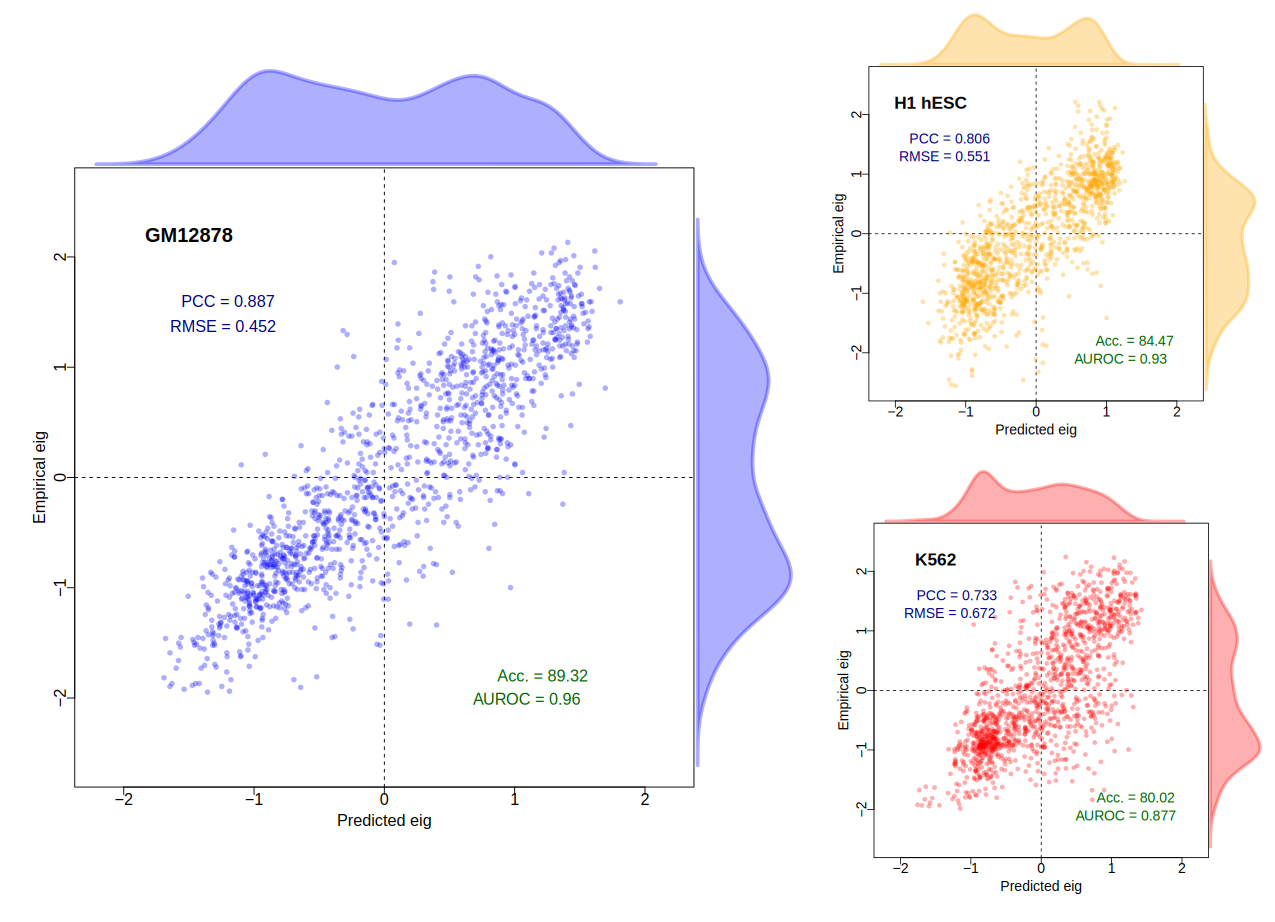
\includegraphics[width=1\textwidth]{figs/f2_full.pdf}
\captionsetup{width=\textwidth}
\caption{ {\bf Accurate models of eigenvector values across three cell
    types.} Predicted eigenvector values are plotted against their
  actual recorded values for each cell type. Evaluation metrics shown
  are Pearson's correlation coefficient (PCC), 
  root mean-squared error (RMSE), and classification evaluators (with
  correct classification defined as either $>0$ in both test
  and training set or both $<0$ --- the top-right and bottom-left
  quadrants of the above plots) accuracy (\% true positives) and area
  under the receiver operating characteristic curve (AUROC). Kernel density estimates describe the
  distribution of their opposite axes.
}\label{fig:modelres}
\end{center} 
\end{figure} 

\vspace{-12pt}
\section{Parsimonious models highlight common features}
\renewcommand*{\thefootnote}{\fnsymbol{footnote}}
Having established that the compartment property of higher order
chromatin structure can be accurately predicted using a feature set of
34 variables, it was then of interest to identify which of these were
most influential in the Random Forest (RF) models. \\

To this end, standard variable importance metrics produced by the RF models,
such as mean decrease in accuracy, can be calculated and compared
between models. However, in this instance there exists strong
multicollinearity between variables, as well as several individual
high correlations between input feature and output eigenvector. For
this reason a form of tuneable regularisation was desirable, allowing
the dense models to be restricted to a small number of influential
features which composed an interpretable model. The graphical LASSO\cite{Friedman2008}
(least absolute shrinkage and selection operator; hereafter glasso)
calculates an estimate analogous to a measure of pairwise conditional
independence between nodes,\cite{Menendez2010} and was selected over competing methods for
several resons: {\small (a)} due to the geometry of
$L_1$-regularisation, the resulting precision matrix is sparse, hence
the glasso can be used to removes conditionally independent variables with respect to a
regularisation parameter; {\small (b)} under Gaussian Markov Random
Field (GRMF) theory, the precision matrix estimate relates to an
interpretable graphical output;\footnote{It should be noted that
in this work, rather than using the resulting sparse inverse
covariance matrix to parameterise a Gaussian graphical model, instead
the glasso is used as a means of feature selection to generate a
non-independent subset of influential variables as input to the RF
model.}  {\small (c)} fast speed of execution.\cite{Hastie2001, Friedman2008} \\

\begin{figure}[H] 
\begin{center}
\vspace{-24pt}
\includegraphics[width=1.05\textwidth]{figs/f3_full.pdf}
\captionsetup{width=\textwidth}
\caption{ {\bf Parsimonious models reveal influential features in
    predicting nuclear architecture} (a) Graphical
  models produced by the glasso algorithm\cite{Friedman2008} for 
  varying regularisation parameter $\lambda$. (b) Corresponding RF results using these reduced feature
  sets as in Fig. \ref{fig:modelres} along with (c) variable
  importance estimates in terms of mean decrease in accuracy
  (see
  Methods \ref{sec:rf}). Full $\lambda$ sequences for K562 and H1 are given in the
  supplementary materials (Figs. \ref{fig:suppGlasso}, \ref{fig:auroc}).
} \label{fig:glasso}
\end{center} 
%\vspace{-12pt}
\end{figure} 

Glasso regularisation was used to produce models with $\approx5$
features and these were then used to retrain Random Forest regression
models (Fig. \ref{fig:glasso}). While in each case the model performance slightly deteriorates with increased
  regularisation, the remaining variables offer insight into the
  primary antecedents of chromosome compartmentalisation in each cell
  type. \\

\begin{wrapfigure}{r}{.4\textwidth}
%\vspace{-14pt}
\includegraphics[width=.4\textwidth]{figs/venn.pdf}
\captionsetup{width=.4\textwidth}
\caption{ {\bf Influential features vary among cell types.}
  Venn diagram showing the intersections of features remaining after regularisation in
  parsimonious models of nuclear architecture (Fig. \ref{fig:glasso}).
}\label{fig:venn}
\vspace{-12pt}
\end{wrapfigure}

Surprisingly, the remaining features in the regularised 
models are largely inconsistent between cell types
(Fig. \ref{fig:glasso}). Two histone marks, H3K4me2 and H3K79me2, are
present in each of the regularised models and another two, H3k27ac and
H3k4me1, remain in both K562 and GM12878 cell type models (Fig
\ref{fig:venn}). The remaining variables were specific to individual
cell type models. By selecting equally-sized random subets of variables, it can be shown that the size of the intersection
between all three sets is significantly larger than would be expected by
chance ($p = 9.6 \times 10^{-3}$), yet overall there remains a
surprising disparity between cell types given the observed
correlations of the response variable (Results \ref{res:corr}). \\

\section{ Invariant regions of higher order structure are better described by locus-level
    features}
The set of matched 1 Mb blocks was then stratified
into regions of low, mid and high variability based on the mean
absolute deviation (MAD) of compartment eigenvectors (see Methods
\ref{meth:strat}). Modelling these regions independently revealed that
low structural variability, or relatively cell type invariant blocks, could be
significantly more accurately predicted relative to high structural variability
regions (GM12878: $t_{16} = 2.1, p = 0.051$, H1: $t_{17}=4.4, p = 3.7 \times 10^{-4}$; K562: $t_{12} = 15, p
  = 3.8 \times 10^{-9}$; Fig. \ref{fig:stratvar}). Additionally, in
  the K562 cell type, the subset of regions conserved with GM12878 and H1 could
  be significantly better predicted than all 1 Mb blocks ($t_{17} =
  7.1, p = 2 \times 10^{-6}$). \\

\begin{figure}[H]
\begin{center}
%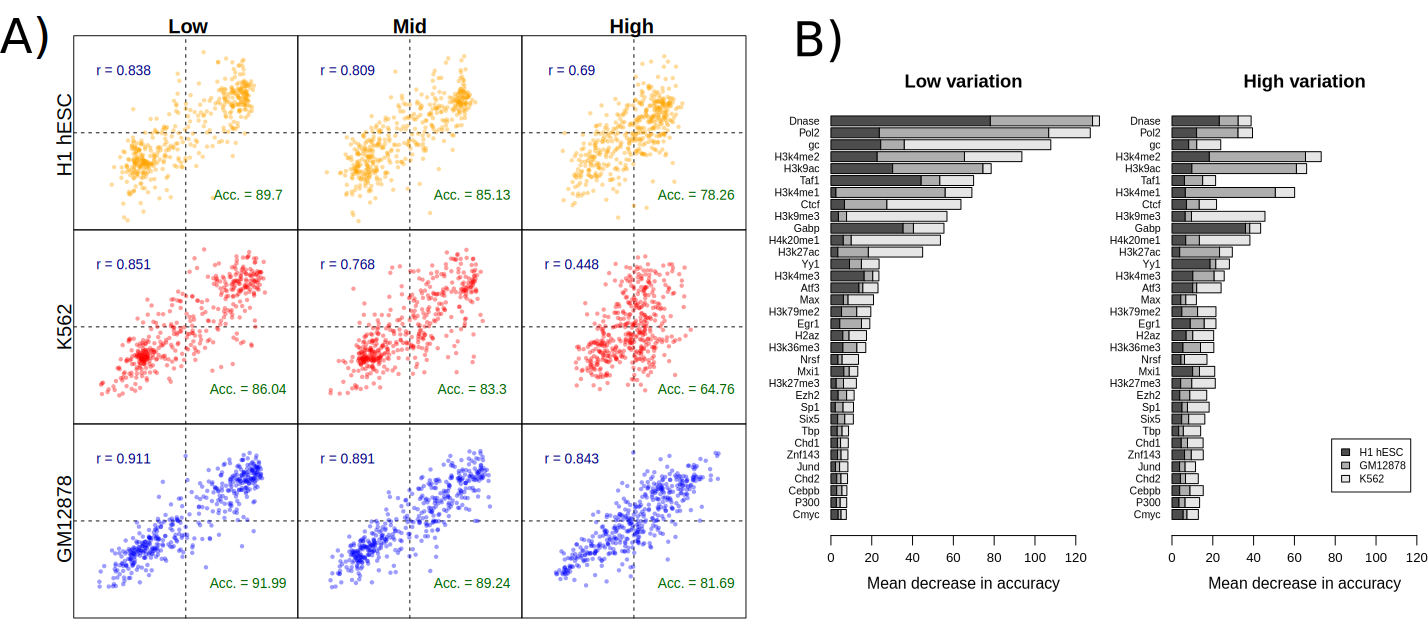
\includegraphics[width=1.1\textwidth]{figs/f4_full.pdf}
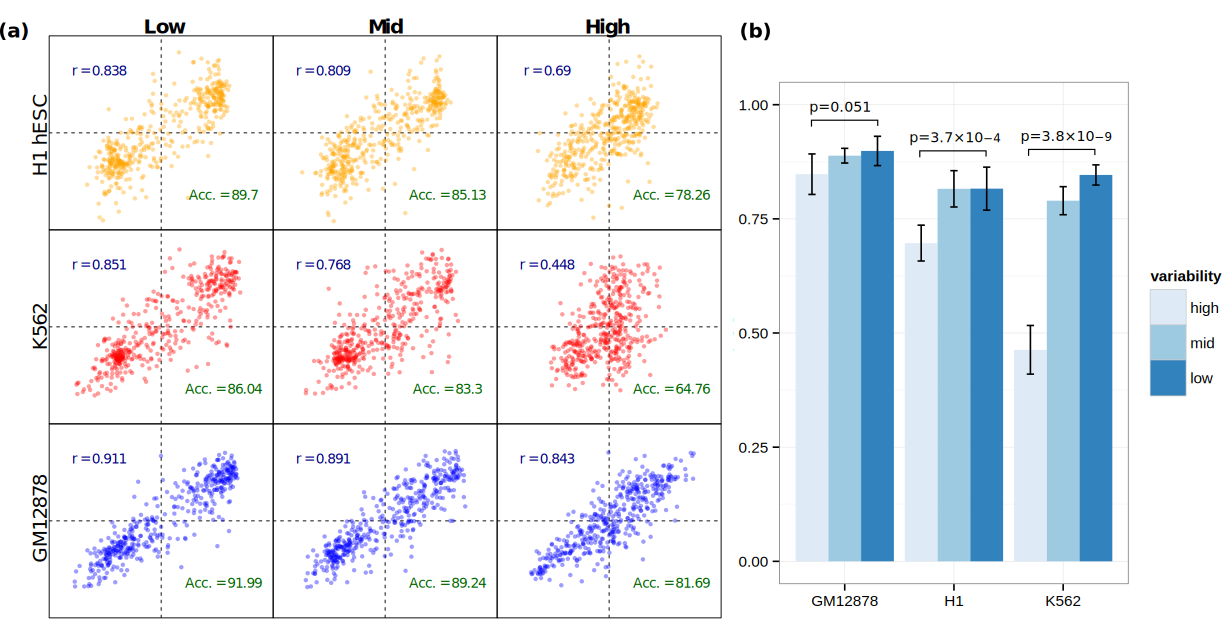
\includegraphics[width=\textwidth]{figs/strat.pdf}
\captionsetup{width=\textwidth}
\caption{ {\bf Regions of variable structure are more difficult to
    model than those that are stable across cell types.}  (a)
  Scatterplots comparing predicted and empirical eigenvector values
  for subsets split by variability. (b) Bar chart showing the
  average Pearson's correlation coefficient (PCC) over all 10 folds,
  with $95\%$ confidence intervals indicated. ``Low''
  variability regions, the third of the 1 Mb bins with the
  lowest median absolute deviation across cell types, proved more
  amenable to predictive modelling in each cell type. 
%B) A stacked bar chart of the
  %relative variable importance of features in the Low variability RF
  %models and high variability RF models in each cell type, ordered by
  %cumulative mean decrease in accuracy in low variability models.
}\label{fig:stratvar}
\end{center} 
\end{figure} 

This result could indicate that there exists a number of genomic sites with a fixed
higher order chromatin state that is well-defined by histone marks,
transcription factors and related components. Conversely, the hard-to-predict variable regions could be those under the influence of
cell type specific factors which are not present in the set of
predictors, or through localised chromatin events. An alternative
interpretation is that the high variability regions are those in which
the principal component is least accurately reflecting columns of the
Hi-C interaction matrix, or those regions most affected by artefacts of
the Hi-C data processing. \\

Significantly invariant blocks (see Methods \ref{meth:strat}) were
tested for a range of potential genomic functional annotation enrichments using the GREAT
tool,\cite{McLean2010} but no significant results were observed
(\emph{data not shown}). \\


% \begin{figure}[H]
% \begin{center}
% \includegraphics[width=1.1\textwidth]{figs/s11.pdf}
% \captionsetup{width=.9\textwidth}
% \caption{ {\bf Applying a model trained in a specific cell type to
%     another human cell type results in a loss of prediction accuracy.}
% Plots are annotated as $M_i \rightarrow F_j$ where $M_i$ is the cell
% type model and $F_j$ is the cell type feature set being passed to the
% model. In all cases, the prediction accuracy on the unseen
% feature set is reduced, however the H1 model performs almost equally
% well with a GM12878 feature set as it does with the matched H1 data.
% }
% \end{center} 
% \end{figure} 
\pagebreak

\section{Models differ between cell types}\label{sec:xapp}
\begin{wrapfigure}{r}{.55\textwidth}
\vspace{-36pt}
\includegraphics[width=.55\textwidth]{figs/xappBars.pdf}
\vspace{-36pt}
\captionsetup{width=.5\textwidth}
\caption{ {\bf Cross-application of models results in decreased
    prediction accuracy} The PCC between predicted and empirical
  eigenvector values is shown (with $95\%$ confidence intervals) for
  models comparing their performance using feature sets from the same
  cell type against those from the other two.
}\label{fig:xapp}
\vspace{-6pt}
\end{wrapfigure}
The cell type specific models of higher order structure were
cross-applied, such that the locus-level chromatin features of one cell
type were used as a feature set in a RF regression model trained in a
different cell type. In each instance of cross-application, the
models' performance in predicting the chromatin state in foreign
cell types decreased (Fig. \ref{fig:xapp}). \\

In each case of cross-application, the results reflect the degree of
cell type specificity of the model (Fig. \ref{fig:modelres}). For
example, GM12878 higher order structure is more accurately predicted by the H1 model
than K562 structure ($t_{10}=14.6,~p = 6 \times 10^{-8}$). Overall, K562 feature sets result in the lowest
prediction accuracies using GM12878 or H1 models
(Fig. \ref{fig:xapp}).

% \section{{\large ``A'' compartments are more centrally located in the nucleus}}
% \begin{figure}[H]
% \begin{center}
% %\includegraphics[width=\textwidth]{figs/s10_full2.png}
% %\includegraphics[width=\textwidth]{figs/sLocale.pdf}
% \includegraphics[width=\textwidth]{figs/locAster.pdf}
% \captionsetup{width=.9\textwidth}
% \caption{ {\bf ``A'' compartments show a tendency to be located more
%     centrally in the inner nucleus relative to ``B'' compartments.}
%   Kernel density estimates show a preference for positive values of
%   eigen in ``inner'' chromosomes (those whose mass was predominantly found in the innermost
%   spherical compartment as determined by Boyle \emph{et al.}\cite{Boyle2001}) and a greater density
%   of negative values in ``outer'' nuclear shells. This was found to be a
%   statistically significant difference in each cell type, with a one-sided K-S test reporting the cumulative
%   density of ``outer'' chromosomes significantly left-shifted relative
%   to ``inner'' chromosomes ($\ast: p<0.05;~\ast\ast: p<5\times10^{-3}$) 
% }
% \end{center} 
% \end{figure} 

\section{Models generalise to unseen chromosomes}

Given that models do not appear to generalise well across cell types, it was of interest to confirm that the models were
not overfitted to the training data. As an example, the
previously-excluded chromosome 21 (see Methods \ref{meth:eigs}) was used as an external validation
set (Fig. \ref{fig:c21}).

\begin{figure}[H]
\begin{center}

\includegraphics[width=1.05\textwidth]{figs/s_c21_v2.pdf}
\captionsetup{width=\textwidth}
\caption{ {\bf Prediction of eigenvectors for a chromosomes whose first principal component
  does not describe its compartmentalisation.}  
(a) The first principal component of the H1 chromosome 21 interaction
matrix is largely explained by the number of restriction sites per
megabase ($\mathrm{R}^2 = 0.65$; \emph{cf}. chromosome 18: $\mathrm{R}^2 <
0.01$). (b) The model prediction of the H1 compartmentalisation
correlates well with other cell types, in most cases above the average
PCC between all autosomal chromosomes. (c) Visual comparison of predicted eigenvector with the same
chromosome in other cell types.
}\label{fig:c21}
\end{center} 
\end{figure} 

The first principal component eigenvector of chromosome 21 in the H1
cell type can be largely explained by the number of restriction enzyme
sites per Mb, whereas this is not the case for other chromosomes
(Fig. \ref{fig:c21}a). This led to chromosome 21 being excluded from
the main analysis (see Methods \ref{meth:eigs}). However, by applying
the RF regression model for H1 developed using other chromosomes to the
features on chromosome 21, new predicted eigenvector values for H1
chromosome 21 were produced (Fig. \ref{fig:c21}c). The predicted
eigenvector values for chromosome 21 in H1 proved much more
similar to eigenvectors from the same chromosome in other cell
types (Fig. \ref{fig:c21}b). Hence this prediction appears to reflect the genuine compartmentalisation of chromosome 21 in H1 with
reasonable accuracy.

\chapter{Discussion}
\section{ Relationship between locus-level chromatin features and higher
order structure} 
The relationship between locus-level chromatin features and higher
order structure remains poorly understood. This work has shown that strong correlations exists between higher order chromosome 
compartmentalisation and aggregate levels of several histone
modifications and DNA binding proteins. \\

Interpretations of the
observed relationship could be either (a) causative, 
whereby specific histone modifications and other bound factors alter nucleosome dynamics and
bring about a more open and active higher order structure or (b)
purely correlative, such that chromatin is organised by latent factors
(such as 
nuclear lamina and nuclear matrix proteins), with large scale active
regions then painted with active marks as a side-effect of
transcriptional activity.\cite{Henikoff2011} A means of distinguishing between these two
explanations could be a biological perturbation study, with specific
factors (e.g. the methyltransferases responsible for H3K4me2 or
H3K79me2) being downregulated in a population of cells
which could then be used for Hi-C analysis. Significant changes to
compartmentalisation would then indicate a causal role for such
factors 
in higher order chromatin structure. Reversing the changes by the addition of these factors to deficient cells would strengthen the case further. \\

Interestingly, the DOT1 histone methyltransferase which methylates H3K79 has
previously been linked with DNA stability in yeast.\cite{Wysocki2005}
A study of the mammalian orthologue DOT1L reported that despite
correlating with transcription, downregulation of this enzyme left most genes
transcribed at their normal rate.\cite{Steger2008a} The same study
linked the ``parallel nature of H3K4 methylation and H3K79
methylation'',\cite{Steger2008a} implicating co-operation with the
other histone mark (H3K4me2) found in all parsimonious models
(Fig. \ref{fig:glasso}). Similarly, factors disporportionately important in the nuclear architecture of a single cell type might be manipulated to study the effects on cell type specific structures.

% The fractal globule model of genome organisation\cite{Mirny2011} proposes a
% hierarchical and self-similar unknotted topology of which 1 to 10 MB compartments are
% likely the highest level of globular organisation that can be
% identified with Hi-C methods.\cite{Dekker2013} The power-law scaling
% of genomic contacts over distance predicted by this model of genome organisation
% enjoys support from a number empirical and theoretical studies (for
% review see Mirny\cite{Mirny2011}), though competing models exist.\cite{Barbieri2012} \\

\section{Implications for models of genome topology}
A previous statistical analysis hypothesised that interphase chromatin
organisation at the megabase scale is driven
by some combination of sequence factors and epigenetic states,
along with the region's position along a chromosome
arm.\cite{Imakaev2012} This type of explanation ties in with the ``dog-on-a-lead'' model of chromosome
topology,\cite{Krijger2013} which states the chromosome
(holding the ``lead'') constrains genomic regions to local areas of
the nucleus, but within those contraints genes and regulatory elements have some
flexibility to locate preferential binding partners.\cite{DeWit2013, Krijger2013}
It goes on to postulate that some regions, such as centromeres, are dominant over their
chromosomal constraints and hence have
disproportionate influence on local genomic interactions. \\

This model of chromosome topology is consistent with the observed
high correlation of compartments across cell types
(Fig. \ref{fig:eigcorr}), with constrained chromosomal territories dominant in
organising the invariant regions (encompassing perhaps three quarters
of the genome) while cell type specific chromatin
states are responsible for the observed variable regions. Indeed, some support
for this hypothesis can be found by contrasting relative variable importance metrics
between high and low variability models (Figs. \ref{fig:stratvar},
\ref{fig:rfimp}), where the predictive power of GC content is decreased in all cell types when
comparing low variation regions with those that are highly
variable. This could also explain
the loss of accuracy during cross application (Fig. \ref{fig:xapp})
and the partial overlap of important features in parsimonious
models (Figs. \ref{fig:glasso}, \ref{fig:venn}). \\

\section{Caveats}
In this work, megabase regions were treated as independent response
variables, though the HMMs designed to call compartment states
highlight that this is an oversimplification (Figs. \ref{fig:states}, \ref{fig:varsignif}). Including adjacent compartment
values as predictive variables yielded significant increases in model
accuracy (Fig. \ref{fig:areg}), but does not aid in the understanding
of the relationship between locus-level features and higher order
chromatin. Another important consideration of the presented models and their
underlying datasets is pervasive multicollinearity, which in
particular limits the power of statistical tools to delineate
individual variable contributions.

\begingroup
\let\clearpage\relax
\chapter{Conclusion} 

We have shown that higher order chromatin structure can be accurately
predicted using aggregate locus-level chromatin features. Of these, H3K4me2 and
H3K79me2 appear to be of particular importance across all cell types. We also note that despite a
general concordance of compartment states across cell types, there
exists a surprising degree of divergence between cell-type specific models, both in terms of relative
variable importance and according to cross-application of feature
sets. These observed differences could be due to a hypothesised
biology of genome topology whereby cell type invariant regions can be
well-defined by locus-level signals, but variable regions may be more
influenced by specific active enhancers and other facets of
transcription activity.
\endgroup

\newpage


%\addcontentsline{toc}{chapter}{Additional figures}
\chapter{Additional figures}
%\setcounter{figure}{0}
%\makeatletter
%\renewcommand{\thefigure}{A\@arabic\c@figure} 

\begin{figure}[H]
\vspace{-36pt}
\begin{center}
\includegraphics[width=.55\textwidth]{figs/corrgram.png}
\captionsetup{width=\textwidth}
\caption{ {\bf General concordance of eigenvectors across cell types.}
  Correlogram showing the mean correlation of eigenvectors across
  selected chromosomes of five human cell types. Pearson's correlation
  coefficient is shown (\emph{upper}) along with kernel density
  estimates of each cell type's eigenvector distribution
  (\emph{diagonal}) and scatterplots comparing megabase blocks from
  each cell type (\emph{lower}).
} \label{fig:corrgram}
\end{center} 
\vspace{-24pt}
\end{figure} 

\begin{figure}[H]
\begin{center}
\includegraphics[width=\textwidth]{figs/states.pdf}
\captionsetup{width=\textwidth}
\caption{ {\bf Eigenvectors and HMM state calls for selected chromosomes
  across three cell types.} $72.6\%$ of HMM state calls (\emph{lower}) are in
agreement across 1 Mb blocks in three human cell types: GM12878, K562
and H1 hESC.
}\label{fig:states}
\end{center}
\end{figure}

\begin{figure}[H]
\begin{center}
\includegraphics[width=.6\textwidth]{figs/s1.pdf}
\captionsetup{width=\textwidth}
\caption{ {\bf Characterisation of open and closed compartment sizes
    in various cell types.}  
Density plots showing the size distributions of open and closed
chromosome compartments. Means are shown with $95\%$ confidence intervals. $n$ refers to the number of 1 Mb blocks
classified as either open or closed.
}
\end{center} 
\end{figure} 

\begin{figure}[H]
\vspace{-12pt}
\begin{center}
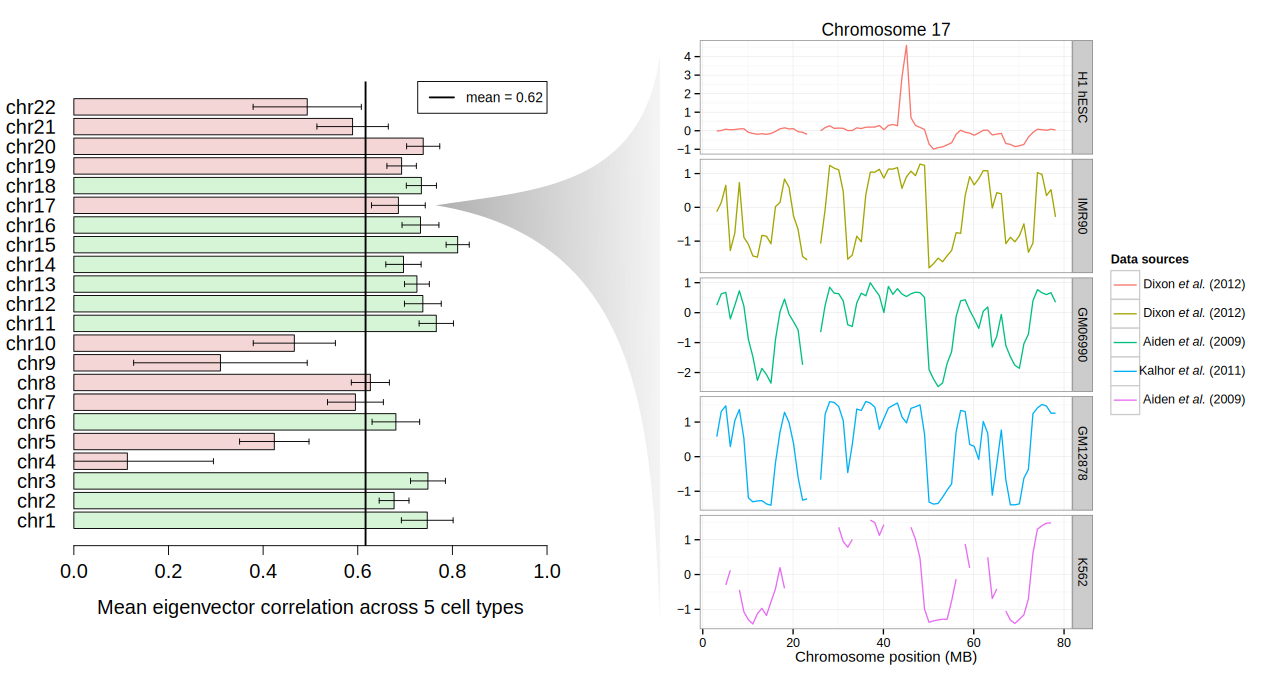
\includegraphics[width=1.08\textwidth]{figs/s2_full.png}
\captionsetup{width=\textwidth}
\caption{ {\bf Selection of correlated chromosomes for modelling.}
Generally those chromosomes whose mean correlation across all 5 cell
types was 1 standard error above the mean were taken forward as
examples of properly-formed PC eigenvectors reflecting A/B
compartmentalisation. Some chromosomes meeting this criterion were
excluded due to obvious aberration or not reflecting the observable
``plaid'' pattern in the normalised interaction matrix, such as
chromosome 17 (\emph{right}).  
}\label{fig:chrselect}
\end{center} 
\end{figure} 

\begin{wide}
\begin{figure}[H]
\begin{center}
\includegraphics[width=1.15\textwidth]{figs/boxcomp.pdf}
\vspace{-.5cm}
\captionsetup{width=\textwidth}
\caption{ {\bf Characterisation of open and closed compartments in
    terms of cell-matched locus level data.} Each variable
  distribution is depicted as a box-and-whisker diagram for open and
  closed megabase blocks. The $y$-axis
  represents the $\log_e$ fold signal change relative to ChIP-Seq
  input control per Mb.
}
\end{center} 
\end{figure} 
\end{wide}

\begin{figure}[H]
\begin{center}
\includegraphics[width=.65\textwidth]{figs/sH1_glasso.pdf}
\includegraphics[width=.65\textwidth]{figs/sK562_glasso}
\captionsetup{width=1\textwidth}
\caption{  {\bf Graphical Lasso $L_1~norm$-based regularisation evolves
    parsimonious graphical models for feature selection.}  Graphical
  models produced by the glasso algorithm are shown for 
  varying regularisation parameter $\lambda$ (\emph{upper}), as in
  Figure \ref{fig:glasso}. Here the results are shown for cell types H1
  (\emph{upper}) and K562 (\emph{lower}).
} \label{fig:suppGlasso}
\end{center} 
\end{figure} 

\begin{figure}[H]
\begin{center}
\includegraphics[width=.75\textwidth]{figs/s4.pdf}
\captionsetup{width=.9\textwidth}
\caption{ {\bf Receiver operating curves for the three cell type
    models at varying levels of regularisation.}  
The receiver operating curves (ROC) are shown for each
  model regularisation (Model 1-4) and for each cell type (see
  Fig. \ref{fig:glasso}). The table (\emph{inset}) gives the
  area under ROC (AUC) value as well as the number of variables
  (nvars) remaining in the each regularised model.
}\label{fig:auroc}
\end{center} 
\end{figure} 

\begin{figure}[H]
\begin{center}
\includegraphics[width=.95\textwidth]{figs/s7_full.pdf}
\captionsetup{width=.9\textwidth}
\caption{ {\bf Random Forest parameters proved largely insensitive to
    parameters ntrees and mtry.}
The number of trees, $ntree$ (A),
was chosen as 200 and the number of variables tested at each
node, $mtry$ (B), was the default value for regression: $n/3 \approx 11$.
}\label{fig:rfparam}
\end{center} 
\end{figure} 

\begin{figure}[H]
\begin{center}
\includegraphics[width=.8\textwidth]{figs/rfimp.pdf}
\captionsetup{width=\textwidth}
\caption{ {\bf Relative variable importance for RF features in models
    built with blocks that are conserved between human cell types (low
    variation) and those that are variable (high variation).} Mean
  decrease in accuracy (Methods \ref{sec:rf}) is calculated for each
  variable in three human cell types and compared between the
  third of regions with the lowest mean absolute deviation
  across cell types (\emph{left}) and the third with the
  highest (\emph{right}).
}\label{fig:rfimp}
\end{center}
\end{figure}

\begin{figure}[H]
\begin{center}
\includegraphics[width=.62\textwidth]{figs/s5.pdf}
\captionsetup{width=\textwidth}
\caption{ {\bf Autoregressive terms increase model accuracy.}  When
  adjacent eigenvector values ($y_{i-1}$, $y_{i+1}$) are used as
  features in predicting the state of a central Mb block ($y_i$) the
  model accuracy greatly improves. This is shown above for the H1 cell
  type, highlighting the known non-independence of adjacent eigenvector values. 
}\label{fig:areg}
\end{center} 
\end{figure} 

% \begin{figure}[H]
% \begin{center}
% \includegraphics[width=\textwidth]{figs/s6.pdf}
% \captionsetup{width=\textwidth}
% \caption{ {\bf Number of NcoI restriction sites vary per MB bin,
%     notably on chromosome 21.}  In two of the main cell types used in
%   this work, Hi-C reads are binned per length of chromosome, while in
%   Kalhor \emph{et al.}\cite{Kalhor2012} reads were binned per given
%   number of restriction sites. The above plot shows how the
%   variability in restriction sites per MB for the restriction enzyme NcoI.\cite{Yaffe2011}
% }
% \end{center} 
% \end{figure}

% \begin{figure}[H]
% \begin{center}
% 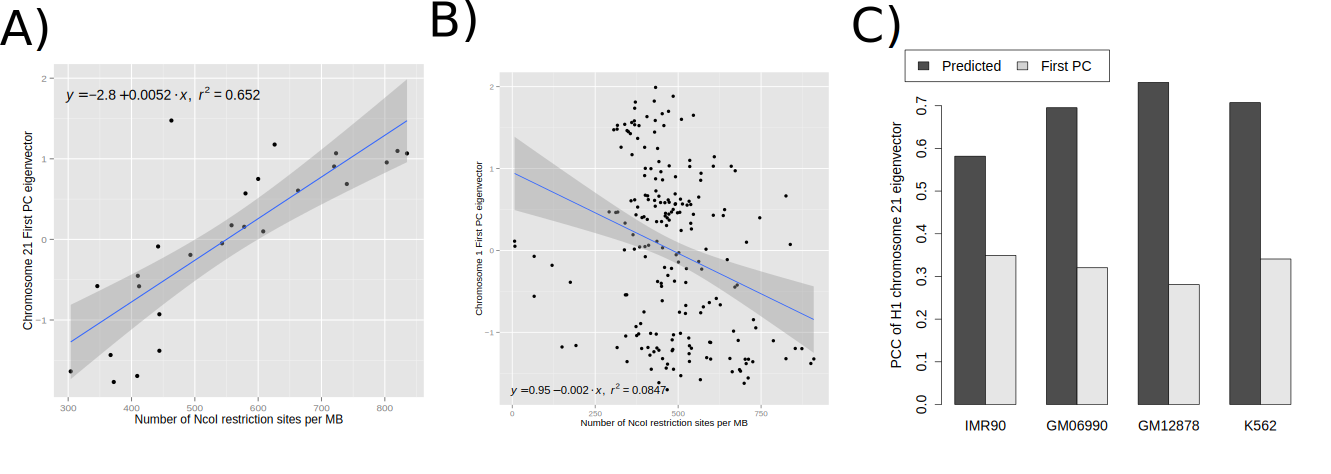
\includegraphics[width=1.1\textwidth]{figs/s8_full.pdf}
% \captionsetup{width=.9\textwidth}
% \caption{ {\bf Restriction sites per MB correlate with H1 first PC in
%     chromosome 21, our model predicts an eigenvector which is more
%     concordant with the other cell types.}  
% }
% \end{center} 
% \end{figure} 



\pagebreak

% \begin{multicols}{2}
% \begin{figure}[H]
% \includegraphics[width=.5\textwidth]{figs/sDiv1.png}
% \end{figure}
% \columnbreak
% \begin{figure}[H]
% \includegraphics[width=.5\textwidth]{figs/sDiv1311.png}
% \end{figure}
% \end{multicols}

% \begin{figure}[H]
% \begin{center}
% \captionsetup{width=.9\textwidth}
% \caption{ {\bf The most divergent and conserved genome compartments
%     across 4 cell types.}  The most variable 1MB block between cell
%   types is shown (\emph{left}) along with annotated EMSEMBL
%   transcripts found within or near the defined region. The same is
%   shown for the most conserved block (\emph{right}).
% }
% \end{center} 
% \end{figure}

\begin{figure}[H]
\begin{center}
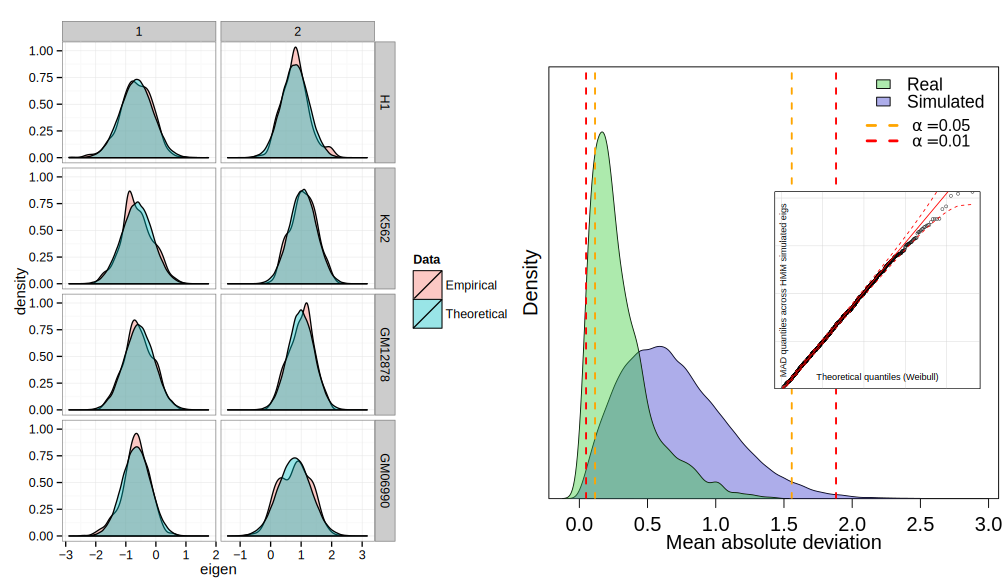
\includegraphics[width=\textwidth]{figs/s13_all.pdf}
\captionsetup{width=\textwidth}
\caption{ {\bf Estimating the significance of median absolute deviations
  observed between eigenvectors across cell types.} Two state normal
HMMs were fit to observed eigenvectors in each cell type (\emph{left})
and the median absolute deviation was calculated at each position. The
distribution of these values was approximated by a Weibull
extreme-value distribution (with $k = 1.87$, $\lambda = 0.76$; QQ-plot
\emph{right, inset}) and the quantiles of this distribution were used
to determine the significance of observed values (\emph{right}).
}\label{fig:varsignif}
\end{center} 
\end{figure} 



%\bibliographystyle{unsrt}
\bibliographystyle{pnas2009}
\begin{footnotesize}
\bibliography{/Users/benmoore/Documents/library}
\end{footnotesize}
\end{document}
